\documentclass[fr]{../../../eplsummary}

\usepackage{../../../eplunits}
\usepackage{../../../eplelec}
\usepackage{circuitikz}

\hypertitle{Circuits électroniques analogiques et digitaux fondamentaux}{5}{ELEC}{1530}
{Antoine Paris}
{Denis Flandre et Jean-Didier Legat}

\paragraph{Notations}
La synthèse suit la notation du livre et du cours.
Un signal $i_C(t)$ est réprésenté mathématiquement
comme ayant une composante constante $I_C$ et une
composante variable $i_c(t)$ de telle sorte que
\[ i_C(t) = I_C + i_c(t). \]
On utilise $I_c$ pour indiquer l'amplitude de
la composante variable $i_c(t)$. 

\part{Dispositifs et circuits de base}
\section{Amplificateurs opérationnels}
Voir synthèse du cours LELEC1370.

\section{Diodes}
\subsection{Diode idéale}
Idéalement, la diode se comporte comme un
interrupteur ouvert quand la tension à ses
bornes est négative et fermé dans le cas
contraire. Le symbole de la diode est quant
à lui donné à la figure \ref{fig:diode-reprensation}.
La courbe courant-tension de la diode idéale est
quant à elle représentée sur la
figure \ref{fig:iv-ideal-diode}. 

\begin{figure}[ht]
	\centering
	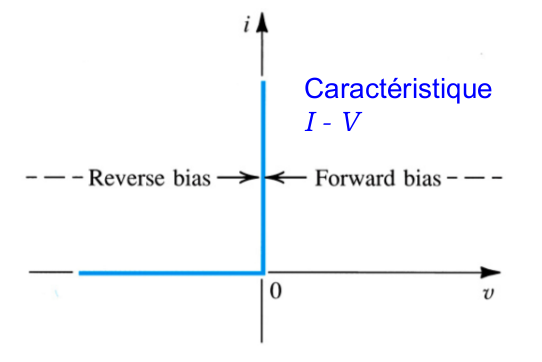
\includegraphics[scale=0.35]{img/iv-ideal-diode.png}
	\caption{Courbe caractéristique d'une diode idéale.}	
	\label{fig:iv-ideal-diode}
\end{figure}

\begin{figure}[ht]
	\centering
	\begin{circuitikz}[american voltages]
		\draw (0,0) to [diode, v^<=$v$, i_=$i$] (4,0); 
	\end{circuitikz}
	\caption{Symbole et conventions de sens pour la diode.
	L'anode est définie comme étant la partie polarisée
	positivement tandis que la cathode est définie comme
	la partie étant polarisée négativement.}
	\label{fig:diode-reprensation}
\end{figure}
   
Formellement, deux configurations sont possibles :
\begin{itemize}
	\item Bloquante (\textit{reverse bias}) : $v < 0 \Rightarrow i = 0$.
	La diode se comporte comme un circuit ouvert ;
	\item Passante (\textit{forward bias}) : $i > 0 \Rightarrow v = 0$.
	La diode se comporte comme un court-circuit.
\end{itemize}

\subsubsection{Application : le redresseur}
En appliquant directement le modèle idéal de la diode,
il apparaît immédiatement que le circuit de la figure
\ref{fig:redresseur} permet de ``couper`` la partie
négative du signal d'entrée $v_I$. Formellement,

\[
v_O = \begin{cases} 
v_I, & \mbox{si } v_I > 0 \\
0,   &\mbox{si } v_I < 0
\end{cases}.
\]

\begin{figure}[ht]
	\centering
	\begin{circuitikz}[american voltages]
		\draw (0,0) to [diode, v^<=$v_D$, i_=$i_D$] (4,0); 
		\draw (0,-2) to [american voltage source, v=$v_I$] (0,0);
		\draw (4,0) to [R, v^<=$v_O$] (4,-2);
		\draw (4,-2) to [short] (0,-2);
	\end{circuitikz}
	\caption{Circuit d'un redresseur.}
	\label{fig:redresseur}
\end{figure}

Cependant, en simulant ce circuit sur SPICE,
on se rend compte que le résultat ne correspond
pas exactement à celui attendu.

\subsection{Modèle empirique pour la diode réelle}
Plusieurs non-idéalités apparaissent en effet : un
décalage en tension en mode passant, un courant
non-nul et une tension de claquage en mode bloquant.
\`{A} haute fréquence, on remarque aussi une certaine
latence lorsque la diode passe du sens passant à bloquant.
D'un point de vue circuit, on représente donc une diode
réelle comme une source de courant en parallèle avec un
condensateur, le tout en série avec une résistance.
La courbe caractéristique d'une diode réelle est représentée
sur la figure \ref{fig:iv-real-diode}.

\begin{figure}[ht]
	\centering
	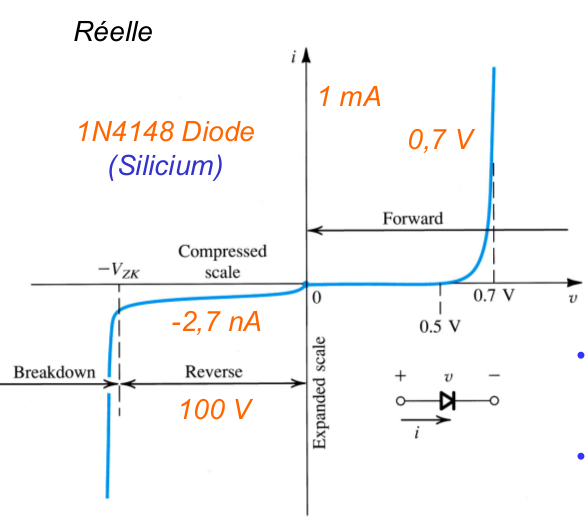
\includegraphics[scale=0.30]{img/iv-real-diode.png}
	\caption{Courbe caractéristique d'une diode réelle.}	
	\label{fig:iv-real-diode}
\end{figure}

En sens passant, on peut approximer le comportement
de la diode par un modèle à chute de tension constante,
dont la courbe caractéristique est représenté sur la
figure \ref{fig:iv-almost-ideal-diode}.

\begin{figure}[ht]
	\centering
	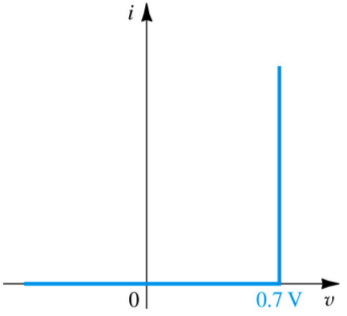
\includegraphics[scale=0.35]{img/iv-almost-ideal-diode.png}
	\caption{Courbe caractéristique d'une diode quasi-idéale.}	
	\label{fig:iv-almost-ideal-diode}
\end{figure}

De manière plus exacte, ce comportement en sens passant
est modélisé de manière empirique par l'équation
\[ i_D = I_S\left(e^{\frac{v_D}{n\cdot V_T}} - 1\right). \]
Dans cette équation, $n$ est constante empirique et
$V_T = \frac{k\cdot T}{q}$ est le coéfficient de température.
Son effet est représenté sur la figure \ref{fig:temp-effect-diode}.
\`{A} \SI{27}{\celsius}, $V_T = \SI{26}{\milli\volt}$.

\begin{figure}[ht]
	\centering
	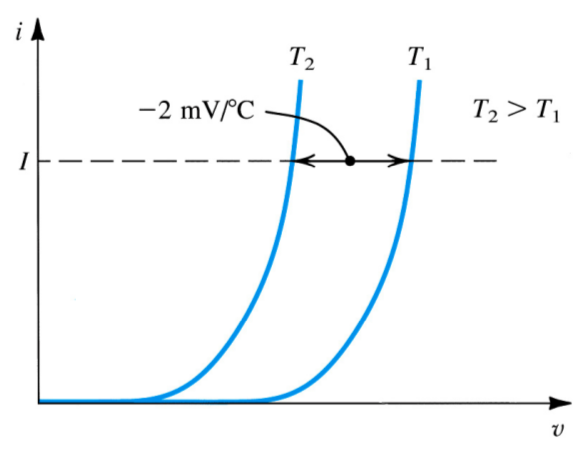
\includegraphics[scale=0.23]{img/temp-effect-diode.png}
	\caption{Effet de la température sur une diode.}	
	\label{fig:temp-effect-diode}
\end{figure} 

\subsection{Modèle petit signal}
\label{subsec:small-signal}
\subsubsection{En général}
Soit un composant électronique dont la relation courant-tension
est donnée par une fonction $f$ non-linéaire telle que $i_D = f(v_D)$.
On peut décomposer $v_D$ en une composante constante $V_D$ et une
composante variable $v_d$ avec $v_d$ très petit.

La série de Taylor de $f(v_D)$ autour du point d'opération DC
$V_D$ est donnée par
\[ i_D = f(V_D) + \left. \frac{\dif f(v_D)}{\dif v_D}\right|_{v_D=V_D}\cdot v_d + \dots \]
où les termes d'ordre supérieurs peuvent être négligés car $v_d$ est
très petit. En décomposant $i_D$ en sa partie constante et sa
partie variable, on peut réecrire l'égalité précédente
\[ I_D + i_d \approx f(V_D) + \left. \frac{\dif f(v_D)}{\dif v_D}\right|_{v_D=V_D}\cdot v_d. \]
En égalant partie constante et partie variable de chaque côté,
on obtient finalement
\begin{align*} 
I_D &\approx f(V_D) \\ 
i_d &\approx \left. \frac{\dif f(v_D)}{\dif v_D}\right|_{v_D=V_D}\cdot v_d.
\end{align*}
On constate donc que la réponse $i_d$ au petit signal $v_d$
est maintenant une fonction linéaire de $v_d$. On défini 
$g_d = 1/r_d$ comme étant la conductance petit-signal
\[ g_d = \left. \frac{\dif f(v_D)}{\dif v_D}\right|_{v_D=V_D}.\]

Une interprétation graphique de ce raisonnement mathématique
est donnée à la figure \ref{fig:small-signal-method-graph}.

\begin{figure}[ht]
	\centering
	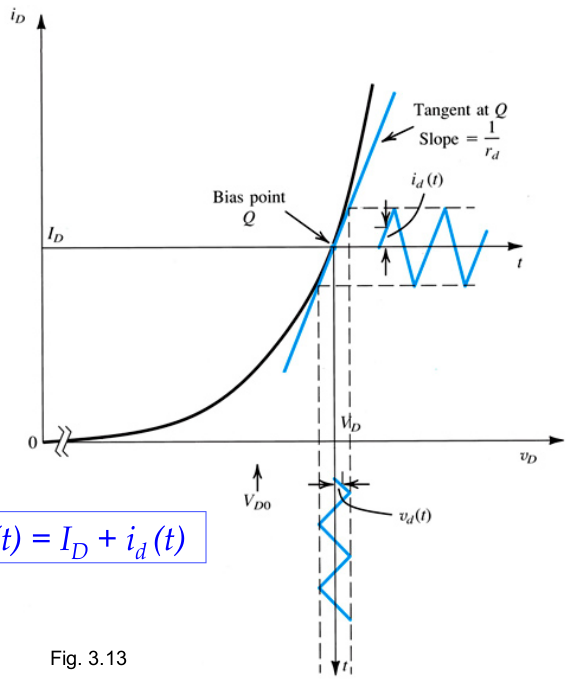
\includegraphics[scale=0.35]{img/small-signal-method-graph.png}
	\caption{Interprétation graphique de la méthode du petit signal.}	
	\label{fig:small-signal-method-graph}
\end{figure}

\subsubsection{Dans le cas de la diode}
Pour une diode, la relation non-linéaire est donnée par
\[ i_D(v_D) = I_s \cdot e^{v_D/V_T}. \] 
% FIX ME : Quid du -1 de la formule donnée plus haut?
En appliquant le même raisonnement que dans le cas général,
on trouve que la résistance petit-signal d'une diode
(aussi appelé sa résistance dynamique) est donnée par
\[ r_d = \frac{V_T}{I_D}. \]
Autrement dit, pour un signal suffisament petit, une
diode se comporte comme une résistance. On dit alors que
le modèle petit signal d'une diode est une résistance.
Il faut cependant faire attention à modifier ce modèle
petit-signal à haute fréquence pour prendre en compte
la capacité parasite de la diode.

% TODO : applications (half-wave-rectifier, full-wave-rectifier,
% peak-rectifier)

\subsection{Diode Zener}
Les diodes Zener sont plutôt utilisé en sens \textit{reverse}
pour avoir une tension de seuil plus élevé (de l'ordre de \SI{6.8}{\volt}).
Le symbole d'une diode Zener est donné à la figure
\ref{fig:diode-zener-representation}.

\begin{figure}[ht]
	\centering
	\begin{circuitikz}[american voltages]
		\draw (0,0) [zDo, v^>=$V_Z$, i_<=$I_Z$] to (4,0);
	\end{circuitikz}
	\caption{Symbole et conventions courant-tension pour une
	diode Zener.}
	\label{fig:diode-zener-representation}
\end{figure}

% TODO : à creuser un peu plus

\subsection{Diodes spéciales}
Une diode \textbf{Schottky} est une diode qui a un seuil de tension très bas
(de l'ordre de 0.3 à \SI{0.4}{\volt}) et un temps de commutation très
faible.

Une diode varicap (pour \textit{variable capacity}) ou  \textbf{varactor}
est une diode qui se comporte comme un condensateur variable.

Une \textbf{photodiode} permet quant à elle de transformer un rayonnement
du domaine optique en un signal électrique.

Enfin, une \textbf{diode électroluminescente} (LED pour
\textit{Light-Emmiting-Diode} en anglais) est une diode
capable d'émettre de la lumière lorsqu'elle est traversée par
un courant.

\section{MOSFET}
\subsection{Structure du transistor MOS}
La structure interne d'un transistor MOS est donnée
à la figure \ref{fig:mos-transistor-structure} dans
le cas d'un transistor NMOS.

\begin{figure}[ht]
	\centering
	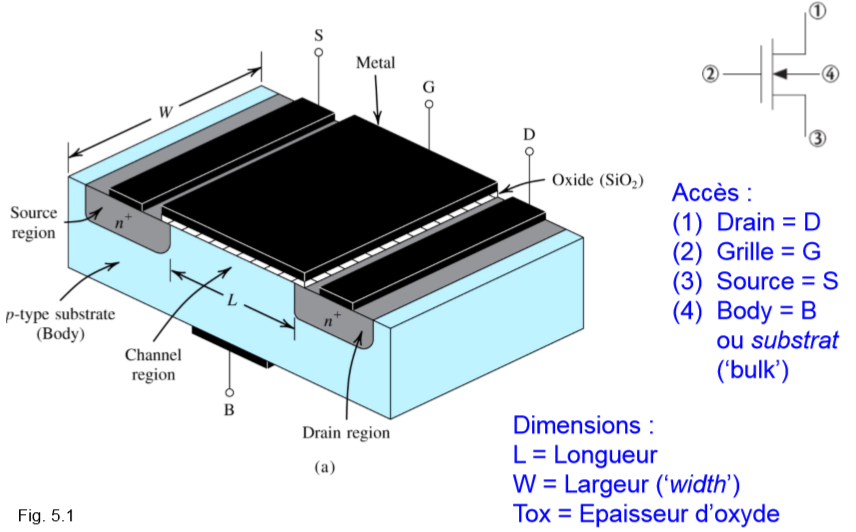
\includegraphics[scale=0.55]{img/mos-transistor-structure.png}
	\caption{Structure physique d'un transistor NMOS.
	Pour un PMOS le substrat est de type $n$ et la source
	et le drain sont de type $p$.}	
	\label{fig:mos-transistor-structure}
\end{figure}

% Explication inspirée de https://www.youtube.com/watch?v=IcrBqCFLHIY

Le substrat est constitué de Silicium (atome tétravalent)
avec un dopage de type $p$ (on ajoute quelques atomes
trivalents). En conséquence, les atomes trivalents ajoutés
ont ce qu'on appelle un ``trou´´. Les électrons des atomes
de Silicium peuvent se déplacer de trous en trous et ainsi
créer un courant.

La source et le drain sont quand à eux constitués de Silicium
avec un dopage de type $n$ (on ajoute quelques atomes
pentavalents). Ce qui signifie qu'en plus des
électrons du Silicium, il y a des électrons libres provenant
des atomes ajoutés. Ces électrons libres créent alors un
courant également.

Lorsqu'aucune tension n'est appliquée sur la grille, certains
électrons libres de la source et du drain vont avoir tendance
à combler les trous adjacents du substrat. Une ``zone de
déplétion'' apparaît alors entre les zones dopées $n$ et
la zone dopée $p$. Dans cette zone de déplétion, il n'y
a plus d'électrons libres dans la zone dopée $n$ et plus de
trous dans la zone dopée $p$. Autrement dit, la zone de
déplétion est chargée négativement du côté dopé $p$. \`{A}
cause de cela, les électrons libres des zones dopées $n$
sont repoussés par la zone dopée $p$ et aucun courant ne
circule entre le drain et la source. 

Si maintenant une tension positive par rapport à la
source est appliquée sur la grille,
les électrons libres de la source vont être attirés vers
la grille et, si cette tension est suffisamment grande, ils
pourront franchir la zone de déplétion et rejoindre le drain
si la tension $v_{DS} > 0$.

Un transistor est donc un interrupteur contrôlé par une
tension.

C'est exactement le même principe pour un transistor
de type PMOS, il suffit d'appliquer le même raisonnement
en inversant les zones dopées $n$ et les zones dopées $p$.

Le symbole d'un transistor de type NMOS est donné à la
figure \ref{fig:nmos-representation} et celui d'un
transistor de type PMOS est donné à la figure
\ref{fig:pmos-representation}.

\begin{figure}[ht]
	\centering
	\begin{circuitikz}[american voltages]
		\draw (0,0) node[nmos](mos) {}
		(mos.base) node[anchor=west] {B}
		(mos.gate) node[anchor=east] {G}
		(mos.drain) node[anchor=south] {D}
		(mos.source) node[anchor=north] {S};
		\ctikzset{tripoles/mos style/arrows};
		\draw (4,0) node[nmos](mos) {}
		(mos.base) node[anchor=west] {B}
		(mos.gate) node[anchor=east] {G}
		(mos.drain) node[anchor=south] {D}
		(mos.source) node[anchor=north] {S};
	\end{circuitikz}
	\caption{Symboles pour un transistor de type NMOS. Par rapport au
	symbole présent sur	la figure \ref{fig:mos-transistor-structure},
	la connexion au substrat a disparu, dans ce cas on considère
	$v_B = v_S$.} 
	\label{fig:nmos-representation}
\end{figure}

\begin{figure}[ht]
	\centering
	\begin{circuitikz}[american voltages]
		\draw (0,0) node[pmos](mos) {}
		(mos.base) node[anchor=west] {B}
		(mos.gate) node[anchor=east] {G}
		(mos.drain) node[anchor=north] {D}
		(mos.source) node[anchor=south] {S};
		\ctikzset{tripoles/mos style/arrows};
		\draw (4,0) node[pmos](mos) {}
		(mos.base) node[anchor=west] {B}
		(mos.gate) node[anchor=east] {G}
		(mos.drain) node[anchor=north] {D}
		(mos.source) node[anchor=south] {S};
	\end{circuitikz}
	\caption{Symboles pour un transistor de type PMOS. Le point noir
	représente le fait que le PMOS est le complémentaire du NMOS.}
	\label{fig:pmos-representation}
\end{figure}

\subsection{Caractéristiques courant-tension}
\subsubsection{Régions de fonctionnement du NMOS}
La sous-section précédente permet de distinguer 3 régions
de fonctionnement du NMOS :
\begin{enumerate}
	\item Si $v_{GS}$ est inférieur à un seuil $V_{tn}$, alors
	les électrons de la source ne pourront pas passer à travers
	la zone de déplétion et le transistor sera en régime
	\textbf{coupé} ou \textbf{cut-off} : $i_D \approx 0$ ;
	\item Si $v_{GS}$ est supérieur au seuil $V_{tn}$ tel que
	$v_{OV} = v_{GS} - V_{tn} > 0$, alors le transistor est en
	régime \textbf{passant} ou \textbf{turned-on} = $i_D > 0$.
	On distingue encore deux cas possibles de régime passant :
	\begin{itemize}
		% TODO : mieux comprendre les deux délimitations ici 
		\item $v_{DS} < v_{OV} \Leftrightarrow v_{GD} > V_{tn}$ :
		régime \textbf{triode}. Dans ce cas, le courant est donné
		par 
		\[ i_D = k'_n\frac{W}{L}\left[v_{OV} - \frac{1}{2}v_{DS}
		\right]v_{DS}; \]
		\item $v_{DS} \geq v_{OV} \Leftrightarrow v_{GD} \leq
		V_{tn}$ : régime \textbf{saturé}. Dans ce cas, le courant
		est donné par
		\[ i_D = \frac{1}{2}k'_n\frac{W}{L}v^2_{OV}. \]
	\end{itemize}
\end{enumerate}

Dans ces équations, $W$ représente la largeur du transistor
et $L$ sa longueur. Il est alors logique que le courant
soit proportionnel à $W$ (plus le ``chemin'' pour les électrons
est large, plus le courant est élevé) et inversement
proportionnel à $L$ (plus le ``chemin'' est long, plus sa
``résistance'' est forte, moins le courant est élevé). $k'_n$
est quand à lui un paramètre lié à l'oxyde utilisé comme
isolant entre la grille et le substrat et est donné par $\mu_n
\frac{\epsilon_{ox}}{t_{ox}}$.

Ces 3 zones de fonctionnement sont représentées schématiquement
sur la figure \ref{fig:iv-nmos}. Sur cette figure, on remarque
que pour des valeurs de $v_{DS}$ faible et pour une valeur
de $v_{GS}$ élevé, le courant $i_D$ est quasi-linéaire, dans
ces conditions, le transistor se comporte donc comme une
résistance.

\begin{figure}[ht]
	\centering
	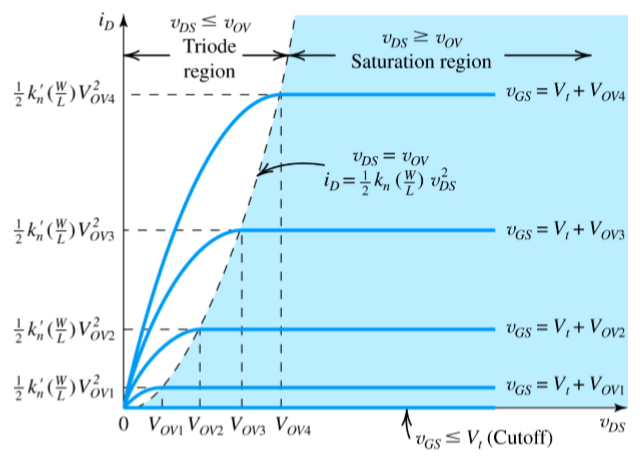
\includegraphics[scale=0.55]{img/iv-nmos.png}
	\caption{Courbes caractéristiques d'un transistor
	NMOS pour différentes valeur de $v_{GS}$.}	
	\label{fig:iv-nmos}
\end{figure}

\paragraph{Effet Early}
En saturation, la réalité ne correspond pas exactement à ce
qu'on peut observer sur la figure \ref{fig:iv-nmos}. On
observe en effet que le courant $i_D$ augmente légèrement avec
$v_{DS}$, on appelle cela l'effet \textbf{Early} ou ``modulation
de longueur de canal''. Lorsqu'on doit tenir compte de cet
effet, on modifie l'équation du courant en saturation
\[ i_D = \frac{1}{2}k'_n\frac{W}{L}v^2_{OV} \cdot (1 + 
\lambda v_{DS}).\]
On défini la tension d'Early $V_A$
\[ V_A = \frac{1}{\lambda} = V'_AL\]
où $V'_A$ est typiquement compris entre
\SI{5}{\volt\per\micro\meter} et \SI{50}{\volt\per\micro\meter}.
Cet effet est représenté sur la figure \ref{fig:early-effect}.

\begin{figure}[ht]
	\centering
	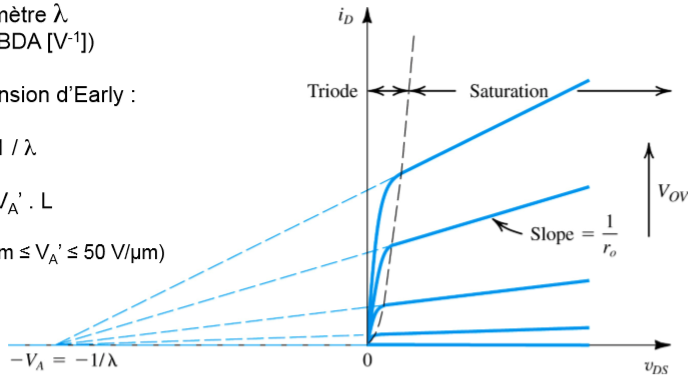
\includegraphics[scale=0.55]{img/early-effect.png}
	\caption{Effet Early.}	
	\label{fig:early-effect}
\end{figure}

\subsubsection{Régions de fonctionnement du PMOS}
Le PMOS étant le complémetaire du NMOS, il fonctionne
exactement de la même façon mais avec la source et le drain
inverse. On peut donc garder les mêmes équations en changeant
$V_{tn}$ par $|V_{tp}|$. La caractéristique courant-tension
d'un transistor PMOS est représenté sur la figure
\ref{fig:iv-pmos}.

\begin{figure}[ht]
	\centering
	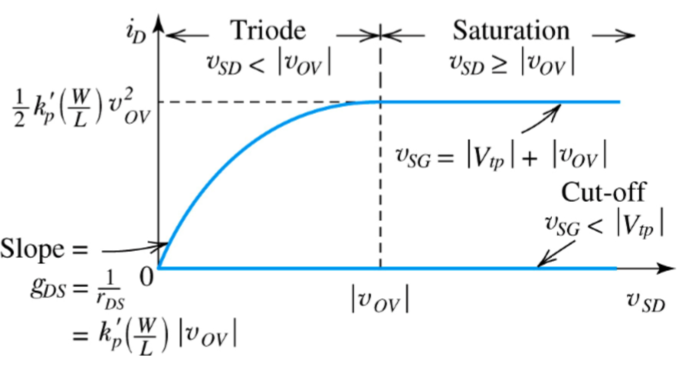
\includegraphics[scale=0.55]{img/iv-pmos.png}
	\caption{Courbe caractéristique d'un transistor PMOS.}	
	\label{fig:iv-pmos}
\end{figure}

\subsection{Amplificateur MOS en grand signal}
On peut construire un amplificateur à l'aide d'un seul
transistor MOS comme indiqué sur la figure
\ref{fig:circ-ampli-mos}.

\begin{figure}[ht]
	\centering
	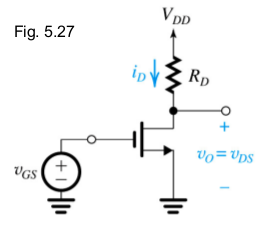
\includegraphics[scale=0.55]{img/circ-ampli-mos.png}
	\caption{Amplificateur MOS.}	
	\label{fig:circ-ampli-mos}
\end{figure}

Analysons ce circuit afin d'obtenir sa caractéristique de
transfert $v_{DS}$ en fonction de $v_{GS}$. La sortie
$v_O = v_{DS}$ du transistor est donnée par $V_DD - R_Di_D$
Premièrement, lorsque $v_{GS} < V_t$, le transistor est
coupé et $i_D = 0$, on a donc $v_{DS} = V_{DD}$. Ensuite,
$v_{GS}$ devient légèrement supérieur à $V_t$ et donc $v_{OV} > 0$
et le courant $i_D \neq 0$. On a donc $v_O = v_{DS} < V_{DD}$
mais $v_{DS} > v_{OV}$ , le transistor est donc en saturation
et on a $v_{DS} = V_{DD} - \frac{1}{2}R_Dk_n(v_{GS}-V_t)^2$
\footnote{Où $k_n = k'n\frac{W}{L}$.}. Si $v_{GS}$ augmente
encore, le transistor passe en régime triode. On obtient
finalement la courbe caractéristique tracée sur la figure
\ref{fig:ampli-mos-carac}.

\begin{figure}[ht]
	\centering
	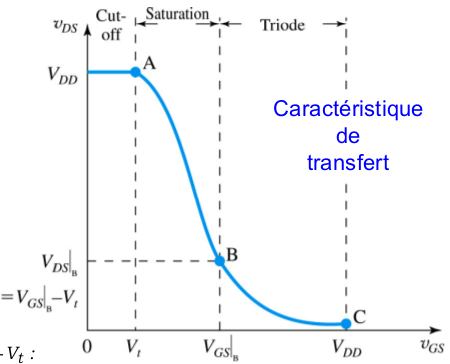
\includegraphics[scale=0.40]{img/ampli-mos-carac.png}
	\caption{Caractéristique de transfert de l'amplificateur MOS.}	
	\label{fig:ampli-mos-carac}
\end{figure}

Le raisonnement effectué pour trouver cette courbe
caractéristique peut également se faire graphiquement,
comme illustré sur la figure \ref{fig:ampli-mos-carac-graph}.

\begin{figure}[ht]
	\centering
	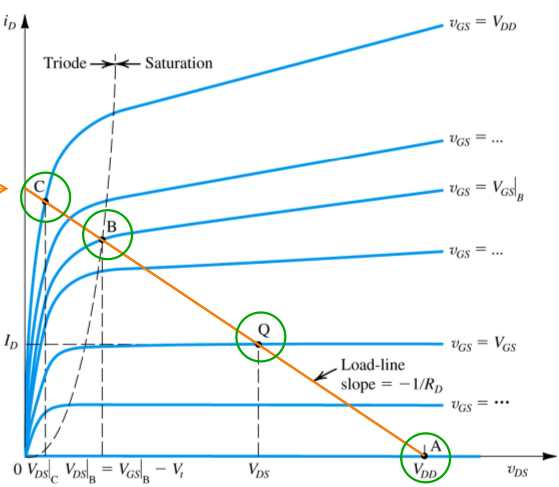
\includegraphics[scale=0.33]{img/ampli-mos-carac-graph.png}
	\caption{Méthode graphique pour trouver la caractéristique de
	transfert de l'amplificateur MOS.}	
	\label{fig:ampli-mos-carac-graph}
\end{figure}

Le gain $A_v$ d'un tel amplificateur est donné par
$\frac{\dif v_{DS}}{\dif v_{GS}}$, il est donc maximum
en saturation (voir figure \ref{fig:ampli-mos-carac})
et vaut
\[ A_v = -k_n\cdot(v_{GS} - V_T)\cdot R_D.\]
On constate que ce gain est d'autant plus grand
que $v_{GS}$ est proche du point $B$ sur la figure
\ref{fig:ampli-mos-carac}. Cependant, il faut
faire attention à ne pas quitter la zone de
saturation sous peine d'arriver dans une zone
non-linéaire et de distordre le signal d'entrée.
Il faut donc placer le point de polarisation DC
entre $A$ et $B$ sur la figure \ref{fig:ampli-mos-carac}
de manière à ce que le petit signal ne dépasse
ni dans la zone coupé (auquel cas le signal serait
écrêté) ni dans la zone triode (auquel cas le signal
serait distordu).

\subsection{Modèle petit signal du transistor MOS}
En effectuant un raisonnement similaire à celui
effectué dans la sous-section \ref{subsec:small-signal}
pour un point de polarisation DC situé dans la zone
de saturation, on trouve que la réponse petit signal
en courant de l'amplificateur MOS est linéaire par
rapport à la tension d'entrée
\[i_d = k_n(V_{GS} - V_T)v_{gs} = g_m\cdot v_{gs}\]
où on défini $g_m$ comme la transconductance
petit signal
\[ g_m = \left.\frac{\delta i_d}{\delta v_{GS}} \right|_{v_{GD} = V_{GS}}.\]

On peut donc maintenant remplacer le circuit
de la figure \ref{fig:circ-ampli-mos} par son
équivalent petit signal (voir figure
\ref{fig:small-signal-mos-ampli}).

\begin{figure}[ht]
	\centering
	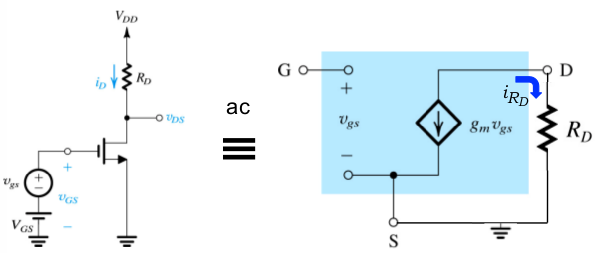
\includegraphics[scale=0.40]{img/small-signal-mos-ampli.png}
	\caption{Circuit équivalent petit signal de l'amplificateur
	MOS.}	
	\label{fig:small-signal-mos-ampli}
\end{figure}

Si on tient compte de l'effet Early, il faut
modifier ce modèle pour include la conductance
dynamique du transistor
\[ g_d = \left.\frac{\delta i_d}{\delta v_{DS}}\right|_{V_{GS}, V_{DS}} = \frac{1}{r_0}\]
de telle sorte que
\[ i_d = g_mv_{gs} + g_dv_{ds}.\]

\begin{figure}[ht]
	\centering
	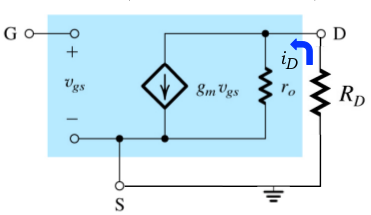
\includegraphics[scale=0.40]{img/ss-mos-ampli-early.png}
	\caption{Circuit équivalent petit signal de l'amplificateur 
	MOS en prenant compte de l'effet Early.}	
	\label{fig:ss-mos-ampli-early}
\end{figure}

% A continuer

\section{Transistor bipolaire (BJT)}
Les symboles d'un transistor bipolaire de type NPN et
de type PNP sont donnés à la figure
\ref{fig:npn-pnp-representation}.

\begin{figure}[ht]
	\centering
	\begin{circuitikz}[american voltages]
		\draw (0,0) node[npn](npn) {}
		(npn.base) node[anchor=east] {B}
		(npn.collector) node[anchor=south] {C}
		(npn.emitter) node[anchor=north] {E};
		\draw (4,0) node[pnp](pnp) {}
		(pnp.base) node[anchor=east] {B}
		(pnp.collector) node[anchor=north] {C}
		(pnp.emitter) node[anchor=south] {E};
	\end{circuitikz}
	\caption{Symbole d'un transistor bipolaire de type NPN à gauche,
	et PNP à droite. $C$ correspond au ``collecteur'', $E$ à l'``émetteur''
	et $B$ à la ``base''.} 
	\label{fig:npn-pnp-representation}
\end{figure}

Le sens des courants $I_E$ et $I_C$ est défini comme allant dans
le sens de la flèche sur le symbole du transistor bipolaire.
$I_B$ est défini comme entrant dans la base pour le NPN et
comme sortant de la base pour PNP. De cette manière, on a toujours
\[ i_E = i_B + i_C. \]

\subsection{Caractéristique courant-tension}
Au vu de la structure d'un transistor bipolaire, on peut
l'approximer par le modèle présenté à la figure
\ref{fig:ebers-moll-model}, appellé modèle Ebers-Moll.

\begin{figure}
	\centering
	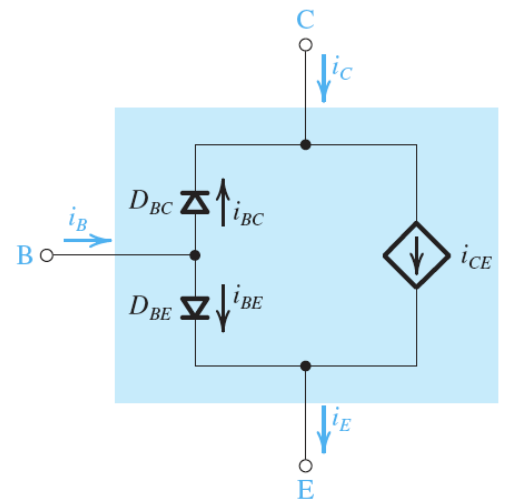
\includegraphics[scale=0.4]{img/ebers-moll-model.png}
	\caption{Modèle Ebers-Moll d'un transistor bipolaire.}
	\label{fig:ebers-moll-model}
\end{figure}

% TODO: développement pour cette équation
On arrive alors une expression générale pour le courant $i_{CE}$
\[ i_{CE} = I_S\left(e^{\frac{v_{BE}}{n_FV_T}} - e^{\frac{v_{BC}}
{n_RV_T}}\right)\left(1-\frac{v_{BC}}{V_A}\right).\]

Pour le transistor bipolaire, on distingue 3
régimes de fonctionnement\footnote{Les conditions sont
ici données pour le NPN. Pour le PNP il suffit d'inverser
les polarités, $v_{BE}$ devient $v_{EB}$, etc.} :
\begin{itemize}
	\item Coupé : les deux diodes sont bloquantes. On a
	donc $v_{BE} <$ \SI{0.5}{\volt} et $v_{BC} <$
	\SI{0.4}{\volt} ;
	\item Actif : la diode $D_{BE}$ est passante 
	($v_{BE} \approx$ \SI{0.7}{\volt}) mais la diode
	$D_{BC}$ est bloquante ($v_{BE} <$ \SI{0.4}{\volt}) ;
	\item Saturation : les deux diodes sont passantes. On a
	donc $v_{BE} \approx$ \SI{0.7}{\volt} et $v_{BC} \approx$
	\SI{0.5}{\volt}.
\end{itemize}

\end{document}
